\chapter{Metodologia de análise de uma Improvisação musical de códigos}\label{cap:metodologia}

Este capítulo busca investigar um método analítico de improvisações que possibilita estruturar \emph{imagens mentais}  e \emph{espaços conceituais} do que está sendo observado como atividade criativa \ver{sec:diferencas}. O \traducao{Quadro Conceitual de Sistemas Criativos}{Creative System Frameworks} \ver{sec:csf} será utilizado como método de análise para uma improvisação de códigos \ver{cap:estudos_de_caso}.

\section{Criatividade e Sistemas Criativos}\label{sec:diferencas}

 Esta teoria supõe uma diferença entre criatividade, Computação criativa, Sistemas criativos e Comportamentos criativos. Sumarizamos estas diferenças  na \autoref{tab:criatividade}.

\begin{table}[!h]
\caption{Definições formais de criatividade por \citeonline[p.~451]{wiggins_framework_2006}}
\small
    \begin{tabular}{ | p{4cm} | p{11.25cm} |}
    \hline 
    \hline 

    \tiny{Criatividade} 
    & \tiny{``A performance de tarefas que, quando executados por um humano, são consideradas criativas''  \tablefootnote{Tradução de \emph{The performance of tasks which, if performed by a human, would be deemed creative.}.}} \\
    \hline

    \tiny{Computação criativa} 
    & \tiny{``O estudo e suporte, através de meios e métodos computacionais, do comportamento exibido por sistemas naturais e artificiais, que são considerados criativos''. \tablefootnote{Tradução de \emph{The study and support, through computational means and methods, of behaviour exhibited by natural and artificial systems, which would be deemed creative if exhibited by humans.}.}} \\
    \hline

    \tiny{Sistemas criativos} 
    & \tiny{``Uma coleção de processos, naturais ou automáticos, que são capazes de alcançarem ou simularem comportamentos que em humanos seria considerado criativo''} \\
    \hline

    \tiny{Comportamento Criativo} 
    & \tiny{``Um ou mais dos comportamentos exibidos por um sistema criativo''\tablefootnote{Tradução de \emph{One or more of the behaviours exhibited by a creative system.}}} \\
    \hline
    \hline
   
    \end{tabular}
\label{tab:criatividade}
\end{table}

%\begin{citacao}
%Por definição, criatividade cria, i.e., produz alguma coisa nova. Mas se estamos comprometidos com uma abordagem mecanicista do mundo -- nenhum milagre é permitido -- iremos acreditar que tudo o que ocorre é, em princípio,  previsível. Iremos acreditar também que qualquer coisa nova deve ser construída de componentes existentes. Isso implica que nada pode ser intrinsicamente novo. \cite[p.~2]{thornton_quantitative_2007}\footnote{Tradução de \emph{By definition, creativity creates, i.e., it produces something new. But if we are committed to a mechanistic account of the world — no miracles allowed — we believe that everything that occurs is predictable in principle. We also believe that any new thing must be constructed from existing components. This implies that nothing can ever be intrinsically new.}}
%\end{citacao}

Por exemplo, a criatividade como uma \emph{prática reflexiva}, descrita por \citeonline[p.~119]{McLean2011}. Ilustra o pintor Paul Klee. Supondo que o artista cria uma imagem mental do que irá fazer (de onde vem essa imagem mental, pode ser uma experiência real, uma lembrança, uma exploração intelectual, uma aula). Decide então esboçar em um desenho. O próximo passo será visualizar o que fez, escolher os gestos apropriados, e readequar outros. Como parte do esboço, pode elaborar seu espectro de cores, e como se organizam no espaço, se são pontos, linhas (com cores quentes ou frias), planos estruturais e questões de luz. Com uma parte decidida, pode ir para o quadro e começar a materializar o esboço. No meio do caminho, percebe que aquilo que foi considerado adequado no esboço, é inadequado para a situação prática, e readequa, direatamente no quadro ou pode voltar ao esboço e redefinir os elementos e depois voltar ao quadro. Após observar o que fez, reage ao resultado dentro de seu próprio sistema estético. Essa reação é acompanhada de uma re-elaboração da imagem mental feita anteriormente, e por novas estratégias de conversão entre a imagem mental e a imagem física. O processo continua até que o ofício seja considerado completo (\emph{obra}). 

Este não é o mesmo processo utilizado pelo(a) improvisador(a)-programador(a). O material, e o objetivo são diversos do(a) artista plástico(a). Seu material é o texto, mas não o texto discursivo, e sim o texto que descreve uma rotina de tarefas computacionais. Seu objetivo não é chegar a uma obra finalizada, mas sim não descontinuar o processo. McLean chama esse processo de programação por bricolagem \ver{fig:processo_criativo}. Em ambos os casos, na prática reflexiva e na bricolagem, são necessários conceitos que suportem a intenção (e vontade) do ofício. Conceitos elaborados através de restrições de idéias podem ser sistematizados, com o auxílio de esquemas visuais. Esta abordagem é muito semelhante à posição defendida por McLean, onde conceitos podem ser representados geometricamente. No caso do(a) improvisador(a)-programador(a), \emph{espaços conceituais} são reelaborados indefinidamente, começando por uma \emph{estratégia transversal}, passando para a observação, reação, e reformulação da imagem mental.

\begin{citacao}
\traducao{A Figura 6.2 $[$\autoref{fig:processo_criativo}$]$ caracteriza a programação por bricolagem como um laço retroalimentado envolvendo o algoritmo escrito, sua interpretação, e a percepção do programador e sua reação do resultado ou comportamento $[$do algoritmo$]$. (\ldots). No começo o programador tem um conceito meio-formado que só atinge consistência interna através do processo de ser expresso como um algoritmo. O laço interno é onde o programador elabora o objetivo de suas imaginações, e o laço externo é onde essa trajetória está fundamentada na pragmática do que elas realmente têm que fazer. Através deste processo ambos algoritmos e conceitos são desenvolvidos até que o programador sinta que um se aplica com o outro, ou de outra forma julga o processo criativo finalizado.
}{
Figure 6.2 characterises bricolage programming as a creative feedback loop encompassing the written algorithm, its interpretation, and the programmer’s perception and reaction to its output or behaviour. (\ldots). At the beginning, the programmer may have a half-formed concept, which only reaches internal consistency through the process of being expressed as an algorithm. The inner loop is where the programmer elaborates upon their imagination of what might be, and the outer where this trajectory is grounded in the pragmatics of what they have actually made. Through this process both algorithm and concept are developed, until the programmer feels they accord with one another, or otherwise judges the creative process to be finished.
}  
\end{citacao}

 \begin{figure}[h]
  \centering
  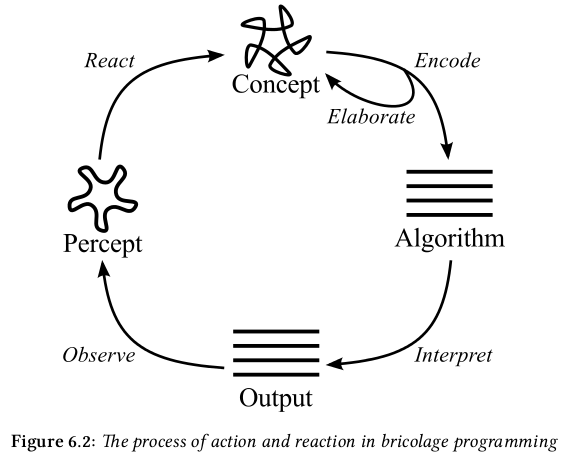
\includegraphics[scale=0.5]{imagens/processo_criativo.png}
  \caption{Modelo de bricolagem para o processo criativo realizado por um artista-programador. \textbf{Fonte}: \citeonline[p.~122]{McLean2011}. }
  \label{fig:processo_criativo}
\end{figure}


\subsection{O programa será transcendido - Língua Artificial é o caminho}\label{sec:imagem_mental}

Definir verbalmente, ``imagem mental'', em termos visuais, estabelece uma relação entre a observação e a verbalização. Por observação não queremos dizer apenas a visão, mas estados conduzidos pela comunicação. Para \citeonline[p.~24]{McLean2011}, imagens mentais se relacionam com quaisquer estados quase-perceptuais: \traducao{Por exemplo o uso de entonação prosódica na fala é \emph{paralinguística}, não inteiramente notada em texto escrito, mas ainda assim simboliza um conteúdo significativo.}{For example the use of prosodic intonation in speech is \emph{paralinguistic}, not entirely notated in written text, yet symbolising meaningful content}. Isto é, na teoria da \emph{Codificação Dual} \apud[p.~25--29]{paivio_dual_1990}{McLean2011}, é estabelecida uma relação de colaboração entre hierarquias de linguagem e códigos de percepção. Esta colaboração estrutura a informação comunicada:

\begin{citacao}
\traducao{Seu $[$Paivio$]$ argumento não é que existem dois códigos, mas sim que existe uma hierarquia de códigos, que se ramificam no topo em códigos lingüísticos discretos e códigos de percepção contínua, que Paivio nomeia como \emph {logogens} e \emph{imagens} respectivamente. (\ldots) \textbf{A explicação oferecida pela teoria da Codificação Dual é que existem sistemas de símbolos distindos, mas integrados, para linguagens e figuras}.}{His contention is not that there are two codes, but rather that there is a hierarchy of code, which branch at the top into discrete linguistic codes and contionuous perceptual codes, which Paivio names \emph{logogens} and \emph{imagens} respectively (\ldots) The explanation offered by Dual Coding Theory is that there are distinct, yet integrated symbol systems for imagery and language.}
\end{citacao}

Para Paivio e McLean,\traducao{humanos são capazes de compreender linguagem enquanto simultaneamente atendem às figuras $[$de linguagem$]$.}{humans are able to comprehend language while simultaneously attending to imagery.}. Por exemplo, quando falamos em \textbf{código de computador}, podemos imaginar um computador, e provavelmente uma pessoa escrevendo um texto. Pode ser também que apenas o computador e o texto escrito apareçam na mente. Pode ser também que apenas o texto escrito, em uma linguagem que não sabemos, seja a imagem mental. Dependendo da experiência acumulada com este objeto \textbf{código}, podemos visualizar outras possibilidades. Mas e o que vêm à mente quando imaginamos algo anterior ao código de computador, sendo que este último materializa a imaginação? ou melhor, quais são os mecanismos que o improvisador utiliza para estimular sua imaginação?

Um sistema integrado entre códigos linguísticos e perceptuais é contextualizado por McLean no caso da improvisação de códigos (\emph{live coding}): se atentarmos para uma partitura-programação, veremos que o programador lida com duas hierarquias. A primeira delas inclue a execução de uma \emph{estratégia transversal}, uma formalização da imagem criada para a notação do código. Isso inclue o comentário, que explica textualmente a imagem e seu resultado; a disposição espacial do código; o destacamento de sintaxe (cores); nomes de variáveis; e nomes de métodos. A segunda hierarquia é descrita através do \emph{Quadro de estruturação das Dimensões Cognitivas da Notação} \apud[p.~95--97]{church_cognitive_2008}{McLean2011}. No caso, é um referencial para a elaboração de novas linguagens, cuja sintaxe pode ser moldada para  atividades específicas (\traducao{Linguagens de Domínio Específico}{DomainSpecific Languages } ou DSL). Para McLean, DSLs ``provêm termos padronizados para descrever demandas particulares em um domínio de uma tarefa'' \ver{tab:dimensoes}. No capítulo anterior, \ver{sec:showusyourscreens}, o item ``O programa será transcendido - Língua Artificial é o caminho.'' trata justamente desta questão, de uma língua que traduza, a partir de algumas restrições, a imagem mental:

\begin{table}[!h]
\caption{Dimensões cognitivas da Notação para linguagens de programação. \textbf{Fonte}: \apud{church_cognitive_2008}{McLean2011}.}
\small
    \begin{tabular}{ | p{7cm}| p{7cm} |}
    \hline 
    \hline 

    \tiny \textbf{Dimensão} & \textbf{Significado} \\
    \hline 
    \hline 

    \tiny \textbf{Abstração}  
    & \tiny \tabletraducao{Disponibilidade de mecanismos de abstração}{Avaliability of abstraction mechanisms} \\
    \hline

    \tiny \textbf{Dependências escondidas}

    & \tiny \tabletraducao{Invisibilidade de ligações importantes entre entidades.}{Invisibility of important links between entities.}\\
    \hline
    
    \tiny \textbf{Compromisso prematuro}  
    & \tiny \tabletraducao{Restrição na ordem de execução das coisas.}{Constraints on the order of doing things.} \\
  \hline

    \tiny \textbf{Notação secundária}  
    & \tiny \tabletraducao{Notação diversa da sintaxe formal.}{Notation other than formal syntax.} \\
    \hline

    \tiny \textbf{Viscosidade}  
    & \tiny \tabletraducao{Resistência à mudança.}{Resistance to change.} \\
    \hline

    \tiny \textbf{Proximidade de mapeamento}  
    & \tiny \tabletraducao{Proximidade de representação para o domínio-alvo.}{Closeness of representation to target domain.} \\
    \hline

    \tiny \textbf{Consistência}  
    & \tiny \tabletraducao{Semânticas similares são expressadas em formas sintáticas similares.}{Similar semantics are expressed in similar syntatic forms} \\
    \hline

    \tiny \textbf{Dispersividade}  
    & \tiny \tabletraducao{Prolixidade da linguagem.}{Verbosity of language.} \\
    \hline

    \tiny \textbf{Tendência ao erro}  
    & \tiny \tabletraducao{Probabilidade de erros.}{Likelihood of mistakes.} \\
    \hline

    \tiny \textbf{Operações mentais difíceis}  
    & \tiny \tabletraducao{Demanda de recursos cognitivos.}{Demand on cognitive resources.} \\
    \hline

    \tiny \textbf{Provisoriedade}  
    & \tiny \tabletraducao{Grau de compromisso com ações e marcos.}{Degree of commitment to actions or marks.} \\
    \hline
    
    \tiny \textbf{Função de expressividade}  
    & \tiny \tabletraducao{medida em que o efeito de um componente pode ser inferida.}{Extent to which the purpose of a component may be inferred.} \\
    \hline
    \hline
   
    \end{tabular}
\label{tab:dimensoes}
\end{table} 

Não explicaremos todas, pois não são dimensões autônomas, o que diverge do foco de nosso trabalho. McLean exemplifica a interdependência entre viscosidade e notação secundária: a possibilidade de diferentes soluções para o mesmo resultado. Isto é, se uma Notação secundária é possível. Por exemplo, em um \emph{patch} de PD, cuja imagem mental é uma onda quadrada. Podemos utilizar objetos nativos ou objetos extendidos \ver{fig:pd}. Uma outra interdependência de dimensões, entre as Operações Mentais Difíceis e a não-Invisibilidade de Dependências Escondidas, é notória do ponto de vista pedagógico. Podem afastar o compositor de seu objetivo musical, mais ou menos estruturado em uma teoria. DSLs como PureData, Max/MSP, CSound, SuperCollider, Tidal, praticam a invisibilidade de dependências em diferentes graus. Porém, entre os improvisadores de código, é considerado virtuosismo o praticante recorrer às Operações Mentais difíceis com o mínimo possível de Invisibilidade de Dependências. Por exemplo, utilizar linguagens de baixo nível como C \ver{sec:concerto}, ou de alto nível como Perl \cite{mclean_hacking_2004} e ainda assim, elaborar sons e imagens de maneira criativa.

\begin{figure}[!h]
  \centering
  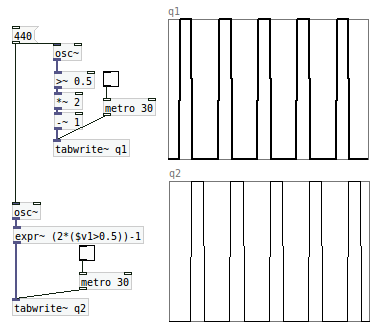
\includegraphics[scale=0.7]{imagens/pd.png}
  \caption{Exemplo de uma caracteristica de viscosidade e notação secundária no PureData. \textbf{Fonte}: autor. }
  \label{fig:pd}
\end{figure}

 
\subsection{Bricolagem como estratégia transversal}\label{sec:tidal}

Vamos ilustrar um pequeno processo da \emph{estratégia transversal} com o \emph{software} Tidal.
Segundo \citeonline[p.~2]{mclean_tidal_2010}, \emph{Tidal} é uma linguagem de composição generativa, onde \traducao{padrões podem ser compostos de numerosos subpadrões em uma variedade de maneiras e para uma profundidade arbitrária, para produzir $[$partes$]$ inteiras complexas de partes simples}{patterns may be composed of numerous subpatterns in a variety of ways and to arbitrary depth, to produce complex wholes from simple parts}. Amostras sonoras representam imagens mentais de suas fontes (por exemplo ``sn'' para \emph{snare}, caixa-clara), com ritmos organizados com o auxílio de símbolos delimitadores de tempo (como espaço, `` ``, e colchetes, ``$[$'',``$]$'', \verb|{| e \verb|}|). Ritmos podem ser revertidos (\verb|rev|), diminuidos e aumentados (\verb|slow|, \verb|density|), iterados (\verb|every|) para recombinação permutação, padrões mais complexos (\verb|can|), como o algoritmode bjorklund que simula ritmos tradicionais\footnote{\cfcite{toussaint_euclidean_2005}}. Efeitos de panoramização, atraso (\emph{delay}), filtros e comunicação de rede. No Exemplo \ref{ex:tidal}. a imagem mental é a demanda da linguagem, que é produzir Música Eletrônica para Dançar.

\begin{citacao}
\traducao{Tidal é uma linguagem de padrões embebida em uma linguagem de programação Haskell, consistindo de representação de padrão, uma biblioteca de padrões geradores e combinadores, um $[$mecanismo$]$ de agendamento de eventos e uma interface para programar ao vivo. Esta é uma extensiva re-escrita de um trabalho anterior introduzido sobre o título \emph{Petrol} $[$\citeonline{mclean_petrol_2010}$]$. Extensões incluem melhoramentos de representação de padrão e um uma integração totalmente configurável do protocolo Open Sound Control $[$\citeonline{osc}$]$ \cite{mclean_tidal_2010}
}
{Tidal is a pattern language embedded in the Haskell programminglanguage, consisting of pattern representation, a library of pattern generators and combinators, an event scheduler and programmer’s live coding interface. This is an extensive re-write of earlier work introduced under the working title of Petrol [15]. Extensions include improved pattern representation and fully configurable integration with the Open Sound Control (OSC) protocol [16]
}
\end{citacao}

\begin{example}{Exemplo de Estratégia Transversal}\label{ex:tidal}

Imagem mental: um \emph{loop} sincopado, mas bastante regular, descrito em um compasso. Em uma ``partitura-mental'', estruturamos o primeiro tempo com um baixo, que volta a tocar na segunda semicolcheia do terceiro tempo. No Segundo tempo, silêncio. No quarto tempo uma caixa aberta:

{%
\parindent 0pt
\noindent
\ifx\preLilyPondExample \undefined
\else
  \expandafter\preLilyPondExample
\fi
\def\lilypondbook{}%

\includegraphics{53/lily-86c766d2-1}%
% eof

\ifx\postLilyPondExample \undefined
\else
  \expandafter\postLilyPondExample
\fi
}

O padrão acima pode ser elaborado em uma voz (\verb|d1|), que redireciona (\$) a função que toca amostras sonoras (\verb|sound|). Esta função lê uma corrente de caracteres (\textbf{string}) separados por um espaço em branco. Espaços em branco são delimitadores temporais. Cada subdivisão temporal é representada por delimitadores como $[$ e $]$. 

\begin{minted}{haskell}
-- Eletronic Dance Music, BPM = 120 
-- tempo 1 - baixo            (bass)
-- tempo 2 - silencio         (silence)
-- tempo 3 - silencio + baixo
-- tempo 4 - caixa            (sn e sn:4)
d1 \$ (sound "bass3 silence [silence bass3] sn:4")
\end{minted}

Sonoramente, é útil para começar. Mas uma Música Eletrônica para Dançar requer mais elementos. Seguiremos com mais dois passos. Podemos complementar os ritmos com uma caixa e um baixos mais secos no segundo e terceiro tempo.

{%
\parindent 0pt
\noindent
\ifx\preLilyPondExample \undefined
\else
  \expandafter\preLilyPondExample
\fi
\def\lilypondbook{}%

\includegraphics{c7/lily-46fd6313-1}%
% eof

\ifx\postLilyPondExample \undefined
\else
  \expandafter\postLilyPondExample
\fi
}

\begin{minted}{haskell}
-- Eletronic Dance Music, BPM = 120 
-- tempo 1 - baixo            (bass)
-- tempo 2 - silencio         (silence)
-- tempo 3 - silencio + house
-- tempo 4 - caixa            (sn e sn:4)
d1 \$ (sound "bass3 sn [silence house] sn:4")
\end{minted}

É possível também fazer com que este padrão reduza seu tempo pela metade a cada quatro tempos, :

{%
\parindent 0pt
\noindent
\ifx\preLilyPondExample \undefined
\else
  \expandafter\preLilyPondExample
\fi
\def\lilypondbook{}%

\includegraphics{2b/lily-de0a8ae3-1}%
% eof

\ifx\postLilyPondExample \undefined
\else
  \expandafter\postLilyPondExample
\fi
}

\begin{minted}{haskell}
-- Eletronic Dance Music, BPM = 120
-- com uma caixa seca no segundo tempo
-- e uma caixa aberta no quarto tempo
-- A cada 4 tempos, o ritmo diminui pela metade 
-- e depois volta ao normal.
d1 \$ every 4 (density 0.5) (sound "bass3 sn [silence house] sn:4")
\end{minted}
\end{example}

Para \citeonline[p.~130]{McLean2011}, esta estratégia criativa, de programar ``no momento'', a partir de um arquivo de texto em branco, com uma imagem mental do resultado sonoro (ou visual), é caracterizada pela  bricolagem. No início do exemplo acima, o programador elabora um meio-conceito do que quer fazer, cuja expressão apenas ganha existência através da codificação \ver{fig:processo_criativo}. As fases de observação, e reação levam o improvisador programador à reconceitualização, e um novo código é escrito. No entanto, ao invés de finalizar, o improvisador segue desenvolvendo.

\section{Sistemas criativos}\label{sec:sistemas}

Para  \citeonline[p.~450]{wiggins_framework_2006}, criatividade pode ser discutida do ponto de vista lógico, orientado geometricamente. A \autoref{eq:vazio} considera a imagem mental de um Universo vazio, e com o máximo potencial de criação. 

\begin{equation}
\mathcal{U} = \emptyset
\end{equation}\label{eq:vazio}

 Wiggins define o Universo de Conceitos (\csf{U}{x}) como um conjunto não estrito dos \emph{Espaços Conceituais} (\csf{C}{x}) de Margaret \citeonline{boden_creative_1990}. Isto é, um Universo de Conceitos a respeito de alguma coisa, no nosso caso da improvisação de códigos \ver{eq:ul}. 

\begin{equation}
\mathcal{U}_\emph{livecoding} = [\mathcal{C}_\emph{Tecelagem}, \mathcal{C}_\emph{Audiovisual}, \mathcal{C}_\emph{Dança} \mathcal{C}_\emph{Música}, \ldots, ?]
\end{equation}\label{eq:ul}

\traducao{Boden concebe o processo de criatividade como uma identificação e/ou localização de novos objetos conceituais em um espaço conceitual.}{Boden conceives the process of creativity as the identification and/or location of new conceptual objects in a conceptual space.}. Uma definição semelhante de \citeonline[p.~2]{thornton_quantitative_2007} reafirma a criação de uma imagem mental de uma \emph{metáfora} (que pode situar sons, palavras, imagens, cheiros,tato,gostos):\traducao{Qualquer ato criativo é fundado na conceitualização ou realização de um ponto dentro de um espaço conceitual particular}{Any creative act is thus founded on conceptualisation or the realisation of a point within a particular ‘conceptual space’}. Neste sentido, selecionamos a imagem mental da metáfora sonora, a partir de um espaço conceitual da Música. Dentro espaço conceitual da Música, selecionamos um específico que vem do \emph{jazz}. Nossa escolha não foi por gosto (ainda que o autor e o orientador gostem), mas sim por ilustrar a intenção de readequação da figura do intérprete concertista para os propósitos do programador \ver{sec:obscurantismo}.  

\subsection{Quadro Conceitual de sistemas criativos}\label{sec:csf}

Uma maneira adequada de descrever um sistema criativo (ou parte dele) considera um \emph{Universo de Conceitos}:

\begin{citacao}
O universo, $\mathcal{U}$, é um espaço multidimensional, no qual dimensões são capazes de representar qualquer coisa, e todos os possíveis conceitos distintos correspondentes àqueles pontos em $\mathcal{U}$ (\ldots) Para tornar a proposta um espaço-tipo possível, permitirei que $\mathcal{U}$ contenha todos os conceitos abstratos, bem como os concretos, e que é possível representar os artefatos tanto completos e incompletos \cite[p.~451]{wiggins_framework_2006}.\footnote{Tradução de \emph{The universe, U, is a multidimensional space, whose dimensions are capable of representing anything, and all possible distinct concepts correspond with distinct points in U. (\ldots) To make the proposal as state-spacelike as possible, I allow that U contains all abstract concepts as well as all concrete ones, and that it is therefore possible to represent both complete and incomplete artefacts}}
\end{citacao}

Wiggins esclarece que Boden não reconhece de forma explícita $\mathcal{U}$, ``ela borra a distinção entre as regras que determinam a adesão do espaço (\ldots) e outras disposições que possam permitir a construção e/ou detecção de um conceito representado por um ponto no espaço'' (\emph{Idem, ibdem}). Espaços conceituais $\mathcal{C}$, finitos ou infinitos são definidos como restrições de um universo $\mathcal{U}$, caracterizando um conjunto não-determinístico de conhecimentos, representações, e conceitos:

\begin{citacao}
\traducao{A noção-chave na teoria de Boden é aquele do espaço conceitual. Enquanto nenhuma definição formal é provida, é comum interpretar esta frase literalmente, tomando o espaço conceitual sendo um espaço de conceitualizações, ou representações de conceitos \cite[p~.7]{thornton_quantitative_2007}.}{The key notion in Boden’s theory is that of the conceptual space. While no formal definition has been provided, it is common to interpret the phrase literally, taking the conceptual space to be a space of conceptualisations or concept representations.}
\end{citacao}

\begin{table}[!h]
\caption{Definições formais do Universo de possibilidades de \citeonline{wiggins_framework_2006}, ou Universo de Conceitos por \citeonline{mclean_music_2006}.}
\small
    \begin{tabular}{ | p{4.25cm} | p{5.25cm} | p{5.25cm} |}
    \hline 
    \hline 

    Representação
    & \tiny{Nome}     
    & \tiny{Significado} \\
    \hline

    $c$
    & \tiny{Conceito} 
    & \tiny{Uma instância de um conceito, abstrato ou concreto \cite{wiggins_framework_2006}}. \\
    \hline

    $\mathcal{U}$
    & \tiny{Universo de Conceitos} 
    & \tiny{Superconjunto não restrito de conceitos. \cite{wiggins_framework_2006}. ``Um universo de todos conceitos possíveis'' \cite{mclean_music_2006} \tablefootnote{Tradução de \emph{A universe of all possible concepts}.}}\\
    \hline

    $\mathcal{L}$
    & \tiny{Linguagem} 
    & \tiny{Linguagem utilizada para expressar regras.} \\
    \hline

    $\mathcal{A}$
    & \tiny{Alfabeto} 
    & \tiny{Alfabeto da linguagen que contêm caracteres apropriadospara expressão das regras} \\
    \hline

    $\mathcal{R}$
    & \tiny{Regras de validação} 
    & \tiny{Validam os conceitos em um universo, se apropriados ou não para o espaço trabalhado.} \\
    \hline

    $[[.]]$
    & \tiny{Função de interpretação} 
    & \tiny{``Uma função parcial de $\mathcal{L}$ para funções que resultam em números reais entre [0, 1] (\ldots) 0.5 $[$ou maior$]$ significa uma verdade booleana e menos que 0.5 siginifica uma falsidade booleana; a necessidade disso para valores reais se tornará clara abaixo'' \cite[p.~452]{wiggins_framework_2006}\tablefootnote{Tradução de \emph{(\ldots) a partial function from $\mathcal{L}$ to functions yielding real numbers in [0, 1]. (\ldots) 0.5 to mean Boolean true and less than 0.5 to mean Boolean false; the need for the real values will become clear below}.}}\\
    \hline

     $[[\mathcal{R}]]$
    & \tiny{Regras de validação} 
    & \tiny{``Uma função que interpreta $\mathcal{R}$, resultando em uma função indicando aderência ao conceito em $\mathcal{R}$''\tablefootnote{Tradução de \emph{A function interpreting $\mathcal{R}$, resulting in a function indicating adherence of a concept to $\mathcal{R}$}}} \\
    \hline

     $\mathcal{C} = [[\mathcal{R}]](\mathcal{U}) $
    & \tiny{Espaço Conceitual} 
    & \tiny{``Todos espaços conceituais são um subconjunto não-estrito de $\mathcal{U}$''\tablefootnote{Tradução de \emph{All conceptual spaces are non-strict subset}.}. Um subconjunto contido em $\mathcal{U}$ \cite{wiggins_framework_2006}. Uma função que interpreta $\mathcal{R}$, resultando em uma função que indica aderência ao conceito em $\mathcal{R}$ \tablefootnote{Tradução de \emph{A function interpreting $\mathcal{R}$, resulting in a function indicating adherence of a concept to $\mathcal{R}$}.} } \\
    \hline

    $\mathcal{T}$
    & \tiny{Regras de detecção} 
    & \tiny{``Regras definidas dentro de $\mathcal{L}$ para definir estratégias transversais para localizar conceitos dentro de $\mathcal{U}$'' \cite{mclean_music_2006}\tablefootnote{Tradução de \emph{Rules defined within $\mathcal{L}$ to define a traversal strategy to locate concepts within $\mathcal{U}$ }}} \\
    \hline

    $\mathcal{E}$
    & \tiny{Regras de qualidade} 
    & \tiny{``(\ldots) conjunto de regras que permitem-nos avaliar qualquer conceito que nós encontramos em $\mathcal{C}$ e determinar sua qualidade, de acordo com critérios que nós considerarmos apropriados'' \cite[p.453]{wiggins_framework_2006}\tablefootnote{Tradução de \emph{(\ldots) set of rules which allows us to evaluate any concept we find in C and determine its quality, according to whatever criteria we may consider appropriate.}}``Regras definidas dentro de $\mathcal{L}$ para avaliar a qualidade ou a desejabilidade do conceito $c$'' \cite{mclean_music_2006}\tablefootnote{Tradução de \emph{Rules defined within $\mathcal{L}$ which evaluate the quality or desirability of a concept $c$.}}}\\
    \hline

    $<<<\mathcal{R}, \mathcal{T}, \mathcal{E}>>>$
    & \tiny{Função de interpretação} 
    & \tiny{Uma regra necessária para definir o espaço conceitual, ``independentemente da ordem, mas também, ficcionalmente, enumerá-los em uma ordem particular, sob o controle de $\mathcal{T}$ -- isto é cricial para a simulação de um comportamento criativo de um $\mathcal{T}$ particular \cite{wiggins_framework_2006} \tablefootnote{Tradução de \emph{We need a means not just of defining the conceptual space, irrespective of order, but also, at least notionally, of enumerating it, in a particular order, under the control of $\mathcal{T}$ -- this is crucial to the simulation of a particular creative behaviour by a particular $\mathcal{T}$.}}. ``Uma função que interpreta a estratégia transversal $\mathcal{T}$, informada por $\mathcal{R}$ e $\mathcal{E}$ . Opera sobre um subconjunto ordenado de $mathcal{U}$ (do qual tem acesso randômico) e resulta em outro subconjunto ordenado de $\mathcal{U}$.''\tablefootnote{Tradução de \emph{A function interpreting the traversal strategy $\mathcal{T}$, informed by $\mathcal{R}$ and $\mathcal{E}$ . It operates upon anordered subset of $mathcal{U}$ (of which it has random access) and results in another ordered subset of $\mathcal{U}$.}}} \\
    \hline
    \hline
   
    \end{tabular}
\label{tab:universodeconceitos}
\end{table}

\citeonline{mclean_music_2006} ainda descreve regras que validam concepções diferentes entre espaços conceituais $\mathcal{C}$ diversos em um Universo de Conceitos $\mathcal{U}$ (ver \autoref{tab:universodeconceitos}). McLean realiza uma comparação entre o \emph{Universo de possibilidades} de Wiggins com o \emph{Modelo de Improvisação} de Pressing \ver{sec:im}. No entanto, McLean argumenta que:

\begin{citacao}
Pressing discute comportamento criativo no contexto do Modelo de Improvisação, e de fato é parte do Quadro conceitual de Sistemas Criativos. (\ldots) Durante a transferência de notação do Modelo de Improvisação para a Ferramenta de Sistemas Criativos, nós consideramos improvisação musical de uma maneira clara e temos uma linguagem comum na qual comparar com outros modelos \footnote{Tradução de \emph{However Pressing does discuss creative behaviour in the context of the IM, and indeed the CSF is in part. (\ldots) In transferring the IM to the notation of the CSF we may consider music improvisation in a clearer manner and have a common language in which to compare it with other models.}}.
\end{citacao}

\section{O modelo de improvisação}\label{sec:im}

Segundo Pressing, o Modelo de Improvisação é ``um esboço para uma teoria geral da improvisação integrada com preceitos da Psicologia Cognitiva (\ldots) teoria do comportamento de improvisação na música'' \cite[p.~2]{pressing_improvisation_1987}. Este modelo será utilizado para especificar elementos de uma performance exemplar, como o caso investigado neste trabalho. Por exemplo, uma improvisação particionada em diferentes sequências pode ser parcialmente mapeada em categorias, como blocos sonoros, referentes conceituais e normas estilísticas, conjuntos de objetivos e processos. Este nos pareceu um modelo mais transparente para o compositor, músico e intérprete. O que não quer dizer que é possível readequar ambos para nosso interesse. Um sumário sobre o modelo de improvisação é apresentado na \autoref{tab:modelo_improvisacao}. Por seu caráter lógico, parece ser uma possibilidade interessante, e assumiremos como tal.

\begin{table}[!h]
\caption{Definições formais do Modelo de improvisação de Jeff \citeonline{pressing_improvisation_1987}, segundo \citeonline[p.~2]{mclean_music_2006}.}
\small
    \begin{tabular}{ | p{6cm} | p{9cm} |}
    \hline 
    \hline 

    \tiny{Representação}   
    & \tiny{Significado} \\
    \hline

    $E'$
    & \tiny{Um bloco de eventos sonoros}\tablefootnote{\emph{A cluster of sound events}.} \\
    \hline

    $K'$
    & \tiny{Uma seqüência de blocos de eventos E, onde um bloco de eventos não se sobrepõe com o seguinte}\tablefootnote{A sequence of E event clusters, where event cluster onsets do not overlap with those of a following one}\\
    \hline

    $I'$
    & \tiny{Uma improvisação, particionada por interrupções em um número de K sequências}\tablefootnote{An improvisation, partitioned by interrupts into a number of K sequences} \\
    \hline

    $R'$
    & \tiny{Um referente opcional, tal como uma partitura ou uma norma estilística}\tablefootnote{An optional referent, such as a score or stylistic norm} \\
    \hline

    $G'$
    & \tiny{Um conjunto de objetivos }\tablefootnote{A set of current goals.} \\
    \hline

    $M'$
    & \tiny{Uma memória de longo prazo}\tablefootnote{Long term memory.} \\
    \hline

    $O'$
    & \tiny{Um conjunto de objetos}\tablefootnote{An array of objects.} \\
    \hline

    $F'$
    & \tiny{Um conjunto de características dos objetos}\tablefootnote{An array of objects Features.} \\
    \hline

    $P'$
    & \tiny{Um conjunto de processos}\tablefootnote{An array of Process} \\
    \hline
    \hline
   
    \end{tabular}
\label{tab:modelo_improvisacao}
\end{table}

\begin{figure}[!h]
  \centering
  \includegraphics[scale=0.7]{imagens/contido.png}
  \caption{Representação da justaposição  entre dois epaços conceituais. A região em marrom representa um grupo de conceitos transitórios, bem como os limites desta transição. \textbf{Fonte}: autor. }
  \label{fig:contido}
\end{figure}

\section{Diagramação dos espaços conceituais}\label{sec:diagrama}

\newcommand{\csfeq}[2]{
\mathcal{#1}_\emph{#2}
}

\newcommand{\unionspaces}[6]{
\csfeq{#1}{#2} = \csfeq{#3}{#4} \bigcup \csfeq{#5}{#6}
}

\newcommand{\listspaces}[9]{
\csfeq{#1}{#2}~=~[\csfeq{#3}{#2},~\csfeq{#4}{#2},~\csfeq{#5}{#2},~\csfeq{#6}{#2},~\csfeq{#7}{#2},~\csfeq{#8}{#2},~\csfeq{#9}{#2}
}

Formalmente, a figura acima pode ser representada como na \autoref{eq:def} , se desconsiderarmos qualquer outros espaços conceituais.

\begin{example}{Representação formal da \autoref{fig:contido}}
\begin{equation}
\unionspaces{C}{Study in Keith}{C}{live coding}{C}{Sun Bears}
\label{eq:def}
\end{equation}
\end{example}

Este grupo também pode ser descrito como uma lista de propriedades como na \autoref{eq:def2}:

\begin{example}{Representação formal das propriedades da \autoref{fig:contido}}
\begin{equation}
\listspaces{C}{SK}{E'}{K'}{I'}{R'}{G'}{M'}{O'}{F'},~\csfeq{P'}{SK}]
\label{eq:def}
\end{equation}
\end{example}
  
Nos diagramas abaixo, $C_\emph{\ldots}$ representa qualquer espaço conceitual abstrato (que pode incluir outro previamente apresentado). Entre os elementos iniciais (raízes, vermelho) e transitórios (nós, azul), ocorrem as ramificações (ramos, linhas pretas), isto é, a exploração de conceitos dentro de outros conceitos. De um lado, a aplicação de regras de validação sobre o universo conceitual da pesquisa (tudo aquilo que foi produzido em dois anos de mestrado) gerou o espaço conceitual desta tese. Estas regras de validação foram, em sua maior parte, os processos de orientação e qualificação. Em outras palavras, \csf{C}{pesquisa}$=[[$\csf{R}{pesquisa}$]]($\csf{U}{pesquisa}$)$.

\begin{example}{Representação do universo conceitual da \emph{pesquisa}}

O Universo de Conceitos da pesquisa, \csf{U}{pesquisa}, é um recorte do universo conceitual da música, \csf{U}{música}:

\begin{tikzpicture}
  [
    grow                    = right,
    sibling distance        = 6em,
    level distance          = 10em,
    edge from parent/.style = {draw, -latex},
    every node/.style       = {font=\footnotesize},
    sloped
  ]
  \node [root] {\csf{U}{Música}}
    child { node [env] {\csf{U}{pesquisa}}
      child { node [env] {\csf{U}{livecoding}}}
    }
    child { node [env] {\csf{C}{\ldots}}};
\end{tikzpicture}

No primeiro capítulo, incluímos um subjconjunto neste Espaço Conceitual da Pesquisa \ver{app:A}). 

\begin{tikzpicture}
  [
    grow                    = right,
    sibling distance        = 6em,
    level distance          = 10em,
    edge from parent/.style = {draw, -latex},
    every node/.style       = {font=\footnotesize},
    sloped
  ]
  \node [root] {\csf{C}{pesquisa}}
    child { node [env] {\csf{C}{livecoding}}
      child { node [env] {\csf{C}{\ldots}}}
      child { node [env] {\csf{C}{ICLC}}}
    }
    child { node [env] {\csf{C}{\ldots}}}; 
\end{tikzpicture}

Podemos inclur elementos históricos, o período transitório entre 1970 e 2000 (\emph{circa}), onde emanciparam as práticas e as regras heurísticas.  

\begin{tikzpicture}
  [
    grow                    = right,
    sibling distance        = 6em,
    level distance          = 10em,
    edge from parent/.style = {draw, -latex},
    every node/.style       = {font=\footnotesize},
    sloped
  ]
  \node [root] {\csf{C}{livecoding}}
    child { node [env] {\csf{C}{Elementos Históricos}}
      child {node [env] {\csf{C}{Proto-História}}}
      child {node [env] {\csf{C}{Manifestos}}}
    }
    child { node [env] {\csf{C}{\ldots}}};
\end{tikzpicture}

Por último, \csf{C}{pesquisa} investiga o \emph{live coding} a partir de um caso específico:

\begin{tikzpicture}
  [
    grow                    = right,
    sibling distance        = 6em,
    level distance          = 10em,
    edge from parent/.style = {draw, -latex},
    every node/.style       = {font=\footnotesize},
    sloped
  ]
  \node [root] {\csf{C}{pesquisa}}
    child { node [env] {\csf{C}{livecoding}}
      child { node [env] {\csf{C}{\ldots}}}
      child { node [env] {\csf{C}{Sessão de Improvisação}}
        child { node [env] {\csf{C}{Study in Keith}}}
        child { node [env] {\csf{C}{\ldots}}}
      }
    }
    child { node [env] {\csf{C}{\ldots}}}; 
\end{tikzpicture}
\end{example}

Por outro lado \csf{C}{Study in Keith} pode ser definido pelo modelo de improvisação de Pressing (\autoref{tab:modelo_improvisacao}, \pageref{tab:modelo_improvisacao}).

\begin{example}{Representação do modelo de improvisação para \emph{Study in Keith}.}
\begin{tikzpicture}
  [
    grow                    = right,
    sibling distance        = 6em,
    level distance          = 10em,
    edge from parent/.style = {draw, -latex},
    every node/.style       = {font=\footnotesize},
    sloped
  ]
  \node [root] {\footnotesize \csf{C}{Study in Keith}}
    child { node [env] {\footnotesize \csf{E'}{Study in Keith}}}
    child { node [env] {\footnotesize \csf{K'}{Study in Keith}}}
    child { node [env] {\footnotesize \csf{I'}{Study in Keith}}}
    child { node [env] {\footnotesize \csf{R'}{Study in Keith}}}
    child { node [env] {\footnotesize \csf{G'}{Study in Keith}}}
    child { node [env] {\footnotesize \csf{O'}{Study in Keith}}}
    child { node [env] {\footnotesize \csf{F'}{Study in Keith}}}
    child { node [env] {\footnotesize \csf{P'}{Study in Keith}}}; 
\end{tikzpicture}
\end{example}

\section{Formalização}\label{sec:formaliza}

O espaço conceitual do \emph{livecoding} é definido como uma função de interpretação das regras de validação (o que pode ser ou não considerado como próprio de uma categorização musical), de gosto (questões de estilo) e de localização transversal de conceitos (conceitos internos que permitem o cruzamento com outros conceitos). As regras de validação foram estudadas neste trabalho como as regras heurísticas do \emph{live coding}. Isto é, que conjunto de métodos são utilizados para caracterizar uma performance de \emph{live coding} como tal? Elementos históricos, e ideológicos (divulgados em manifestos), são levantados para responder esta pergunta. Por outro lado, este estudo abandonou a investigação das regras de gosto, tema que pode ser melhor explorado em trabalhos posteriores, a partir de \citeonline{janotti_jr._a_2003,sa_musica_2006,sa_se_2009}. A tarefa de localização transversal de conceitos é trabalhada no último capítulo. O espaço conceitual de \emph{Study in Keith} está contido no espaço conceitual do \emph{live coding} através da união entre os conceitos deste último, com os espaços conceituais dos concertos \emph{Sun Bears}, de Keith Jarret, misturados. No entanto o espaço conceitual não será investigado em sua totalidade, e sim apenas uma sonoridade.